% =====================================================================
%  NEW SLIDES FOR REVIEW II  --  paste into the deck
%
%  Placement: insert BOTH frames immediately AFTER the existing
%  "Finding 2: No Univariate Progression Signal" slide (slide 26) and
%  BEFORE "Team Responsibilities" (slide 27). Numbered 3 and 4 so that
%  nothing already in the deck has to be renumbered.
%
%  Images: copy these two files next to the .tex (or into your Overleaf
%  project) from
%      derivatives/REVIEW2_FINDINGS/fig_complementarity.png
%      derivatives/REVIEW2_FINDINGS/fig_reliability.png
%
%  Requires only graphicx + booktabs, both already in the preamble.
% =====================================================================


% ---------------------------------------------------------------------
\begin{frame}{Finding 3: The Biomarkers Are Not Redundant}

\begin{center}
  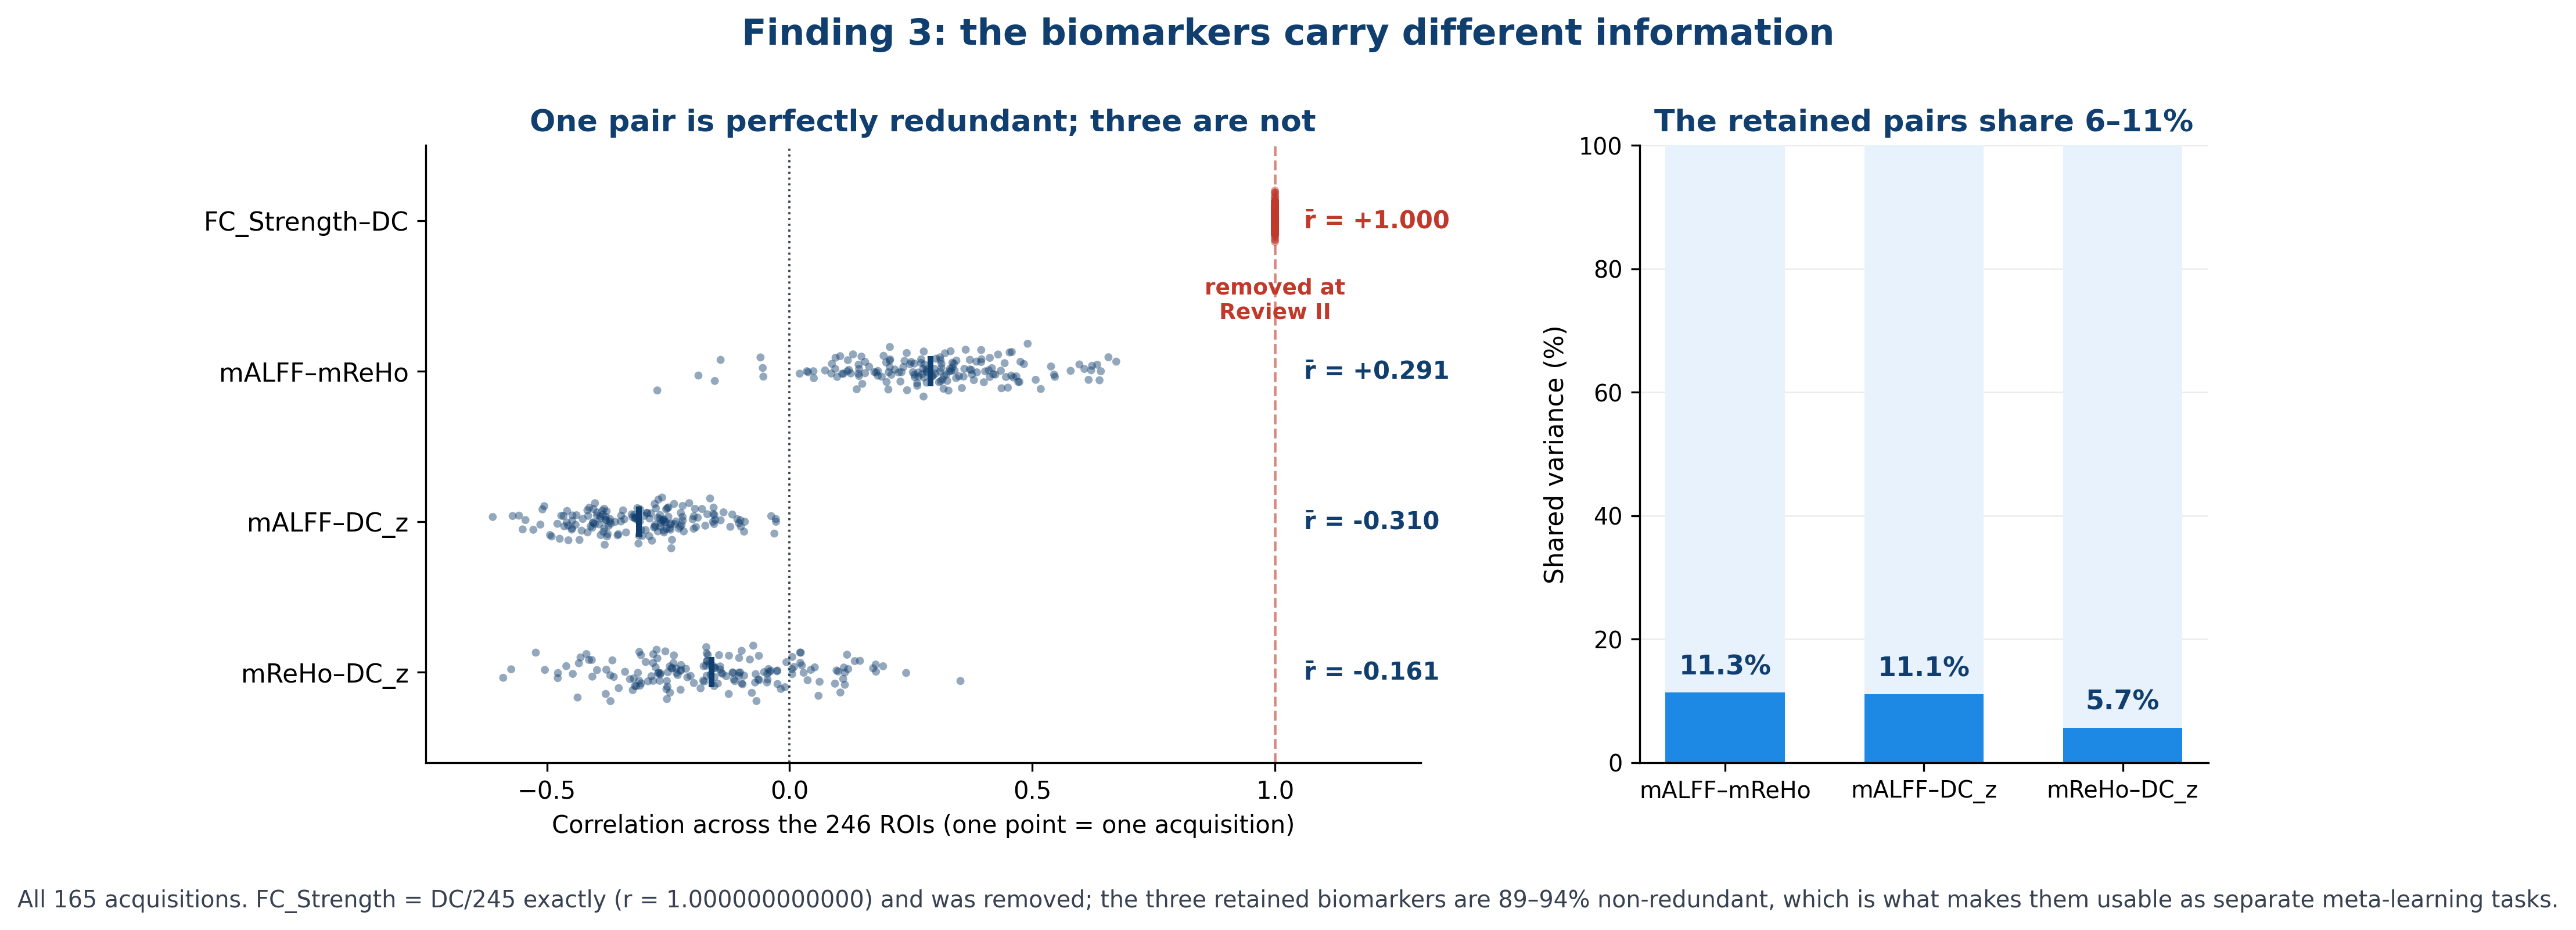
\includegraphics[width=0.96\textwidth]{fig_complementarity.png}
\end{center}

\vspace{-0.2cm}
\begin{columns}[T]
\begin{column}{0.52\textwidth}
\footnotesize
\begin{tabular}{lr}
\toprule
\textbf{Pair} & \textbf{Shared variance} \\
\midrule
FC\_Strength -- DC & 100\,\% \quad (removed) \\
mALFF -- mReHo     & 11.3\,\% \\
mALFF -- DC$_z$    & 11.1\,\% \\
mReHo -- DC$_z$    & \phantom{0}5.7\,\% \\
\bottomrule
\end{tabular}
\end{column}
\begin{column}{0.46\textwidth}
\footnotesize
\begin{itemize}
  \item The three retained biomarkers are \textbf{89--94\,\% non-redundant}.
  \item Measured on all 165 acquisitions, across the 246 regions.
  \item Negative mALFF--DC$_z$: strong local amplitude goes with
        \emph{lower} degree centrality.
\end{itemize}
\end{column}
\end{columns}

\vspace{0.15cm}
\begin{block}{Why this matters for G1}
Gap G1 assumes the biomarkers must be modelled \emph{jointly}. That is now
measured, not assumed: one pair was perfectly redundant and was removed; the
rest are near-independent, so they are usable as separate meta-learning tasks.
\end{block}

\end{frame}


% ---------------------------------------------------------------------
\begin{frame}{Finding 4: The Features Are Reproducible and Plausible}

\begin{center}
  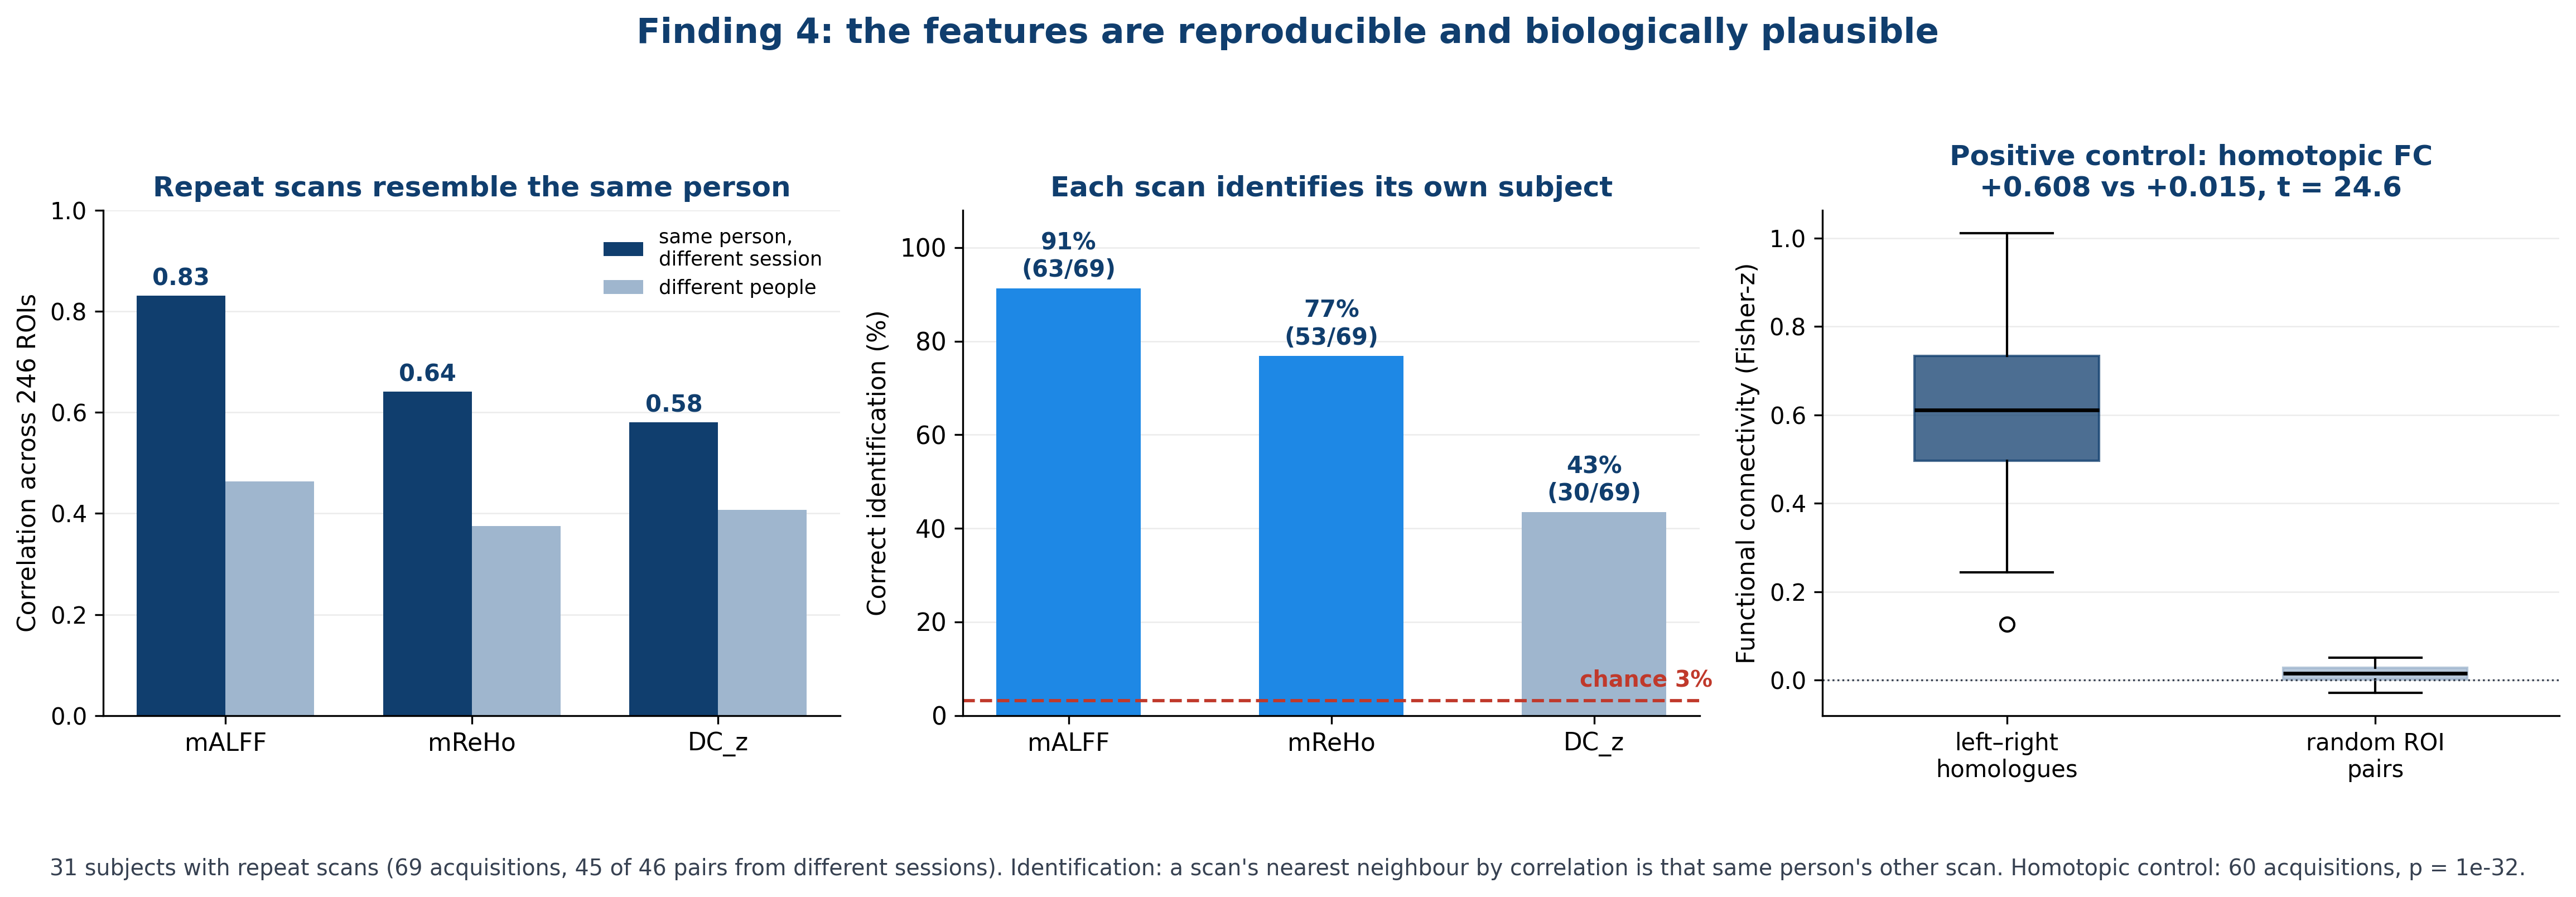
\includegraphics[width=0.98\textwidth]{fig_reliability.png}
\end{center}

\vspace{-0.15cm}
\begin{columns}[T]
\begin{column}{0.54\textwidth}
\footnotesize
\begin{tabular}{lrrr}
\toprule
 & \textbf{Same} & \textbf{Diff.} & \textbf{ID} \\
 & \textbf{person} & \textbf{people} & \textbf{acc.} \\
\midrule
mALFF    & 0.83 & 0.46 & \textbf{91\,\%} \\
mReHo    & 0.64 & 0.38 & 77\,\% \\
DC$_z$   & 0.58 & 0.41 & 43\,\% \\
\bottomrule
\end{tabular}

\vspace{0.1cm}
{\scriptsize 31 subjects with repeat scans; chance = 3\,\%.}
\end{column}
\begin{column}{0.44\textwidth}
\footnotesize
\begin{itemize}
  \item \textbf{45 of 46} repeat pairs are from \emph{different sessions}:
        this is between-session reliability, not same-session.
  \item Homotopic FC $+0.608$ vs $+0.015$ for random pairs
        ($t = 24.6$).
  \item Reliability ranking: mALFF $>$ mReHo $>$ DC$_z$.
\end{itemize}
\end{column}
\end{columns}

\vspace{0.15cm}
\begin{block}{Two independent checks that the pipeline produced real signal}
A scan identifies its own subject 91\,\% of the time against 3\,\% chance, and
the pipeline recovers left--right homotopic connectivity, the most replicated
effect in resting-state fMRI. Neither check uses the stage labels.
\end{block}

\end{frame}


% =====================================================================
%  ADD THESE TWO BULLETS TO "Backup: Data Limitations" (slide 32)
% =====================================================================
%
% \item \textbf{Residual motion in the features:} after 27 regressors,
%       129/246 (mALFF) and 131/246 (mReHo) regions still correlate with
%       mean FD at $p<0.05$ (chance $\approx$ 12). Framewise displacement
%       must enter the model as a covariate; DC$_z$ is less affected
%       (39/246).
%
% \item \textbf{Site is concentrated where it hurts:} 14 sites. One site
%       contributes 40\,\% of all AD scans and two contribute 68\,\%,
%       while no single site exceeds 19\,\% of CN. Any CN--AD contrast is
%       partly a site contrast; harmonisation or a site covariate is
%       needed before Module 4.
%
% =====================================================================


% ---------------------------------------------------------------------
%  OPTIONAL THIRD SLIDE -- answers "why 246 regions?"
%  Place right after the "The Brain Atlas: 246 Regions" slide (slide 9),
%  or hold it in Backup and show it only if the panel asks.
% ---------------------------------------------------------------------
\begin{frame}{Why 246 Regions?}

\begin{center}
  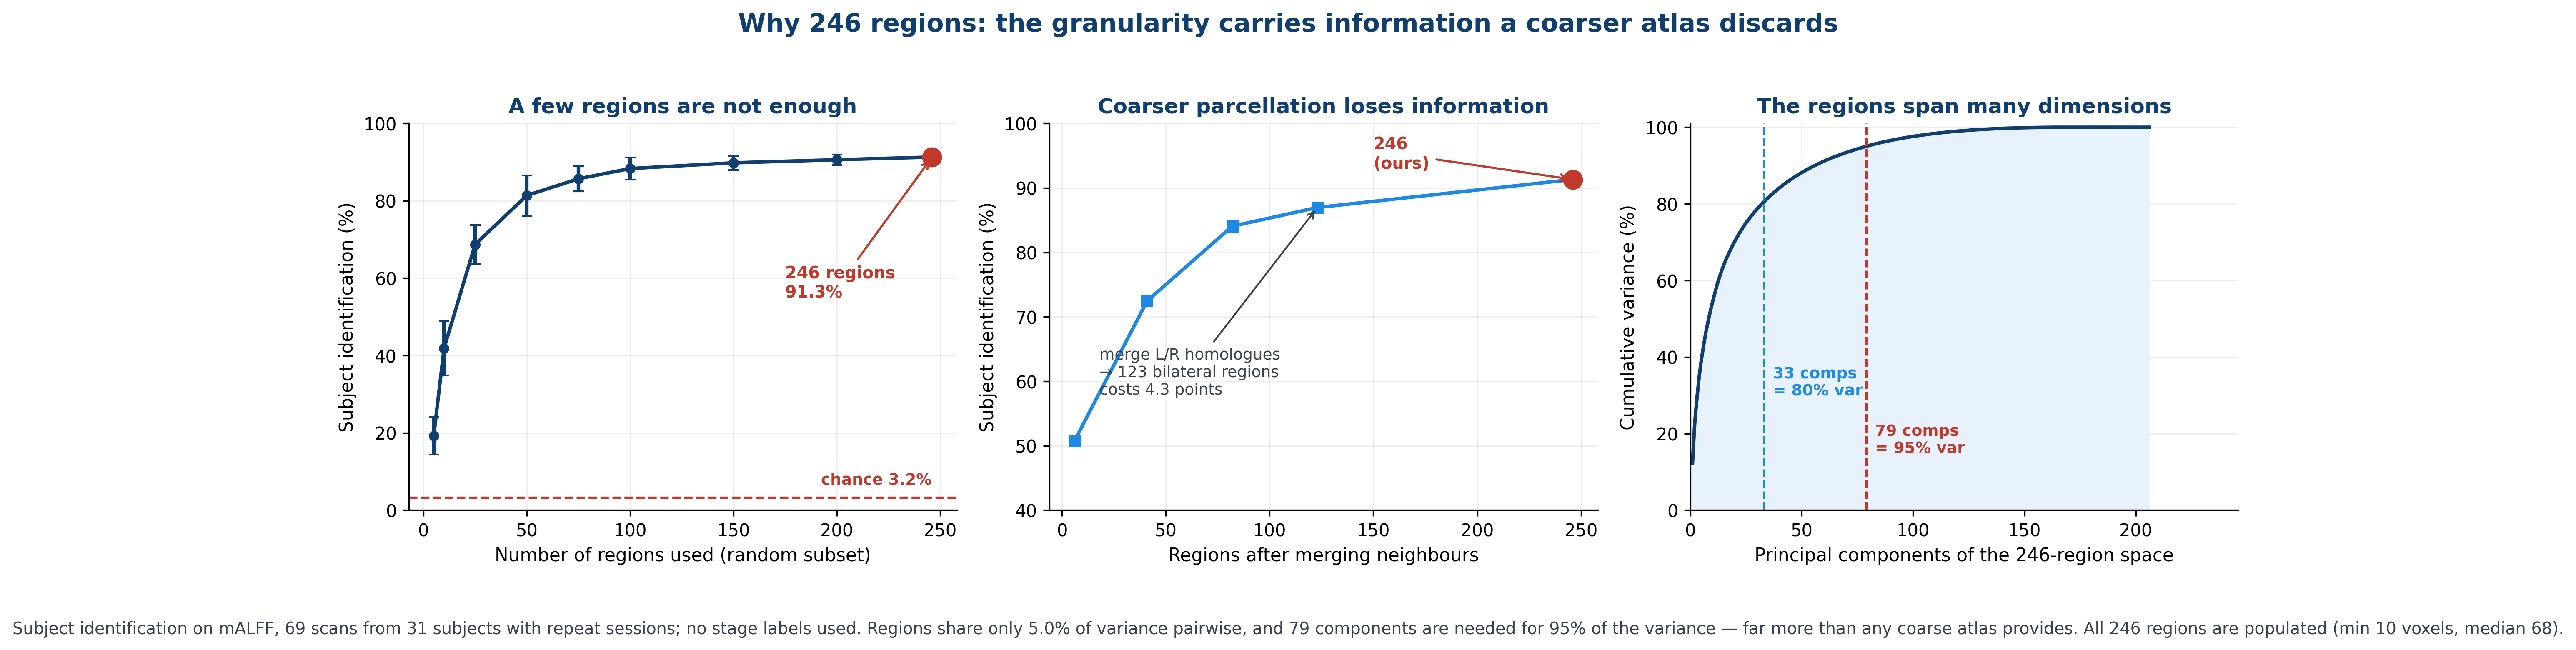
\includegraphics[width=0.99\textwidth]{fig_atlas_granularity.png}
\end{center}

\vspace{-0.1cm}
\begin{columns}[T]
\begin{column}{0.47\textwidth}
\footnotesize
\begin{tabular}{lr}
\toprule
\textbf{Parcellation} & \textbf{Identification} \
\midrule
\textbf{246 (Brainnetome)} & \textbf{91.3\,\%} \
123 (bilateral merge)      & 87.0\,\% \
\phantom{0}82              & 84.1\,\% \
\phantom{0}41              & 72.5\,\% \
\phantom{00}6              & 50.7\,\% \
\bottomrule
\end{tabular}
\end{column}
\begin{column}{0.51\textwidth}
\footnotesize
\begin{itemize}
  \item \textbf{Every} coarsening we tested loses accuracy.
  \item Merging left/right homologues alone costs 4.3 points:
        hemispheric asymmetry is real information.
  \item Regions are not duplicates: 5.0\,\% shared variance pairwise;
        79 components needed for 95\,\% of variance.
  \item Resolves hippocampus (4 subregions) and amygdala (4) --
        a 90-region atlas does not.
\end{itemize}
\end{column}
\end{columns}

\vspace{0.1cm}
\begin{block}{What this does and does not show}
It shows the 246-region granularity carries information that coarser schemes
discard, and that no region is empty (min 10 voxels). It does not claim 246 is
optimal -- that needs the trained model to test.
\end{block}

\end{frame}


% =====================================================================
%  ATLAS JUSTIFICATION -- the "complete feature-extraction space" framing
%  Main slide: place right after "The Brain Atlas: 246 Regions" (slide 9).
%  The two detail slides below belong in Backup.
% =====================================================================

\begin{frame}{Why the Full 246-ROI Space Is Retained}

\begin{columns}[T]
\begin{column}{0.46\textwidth}
  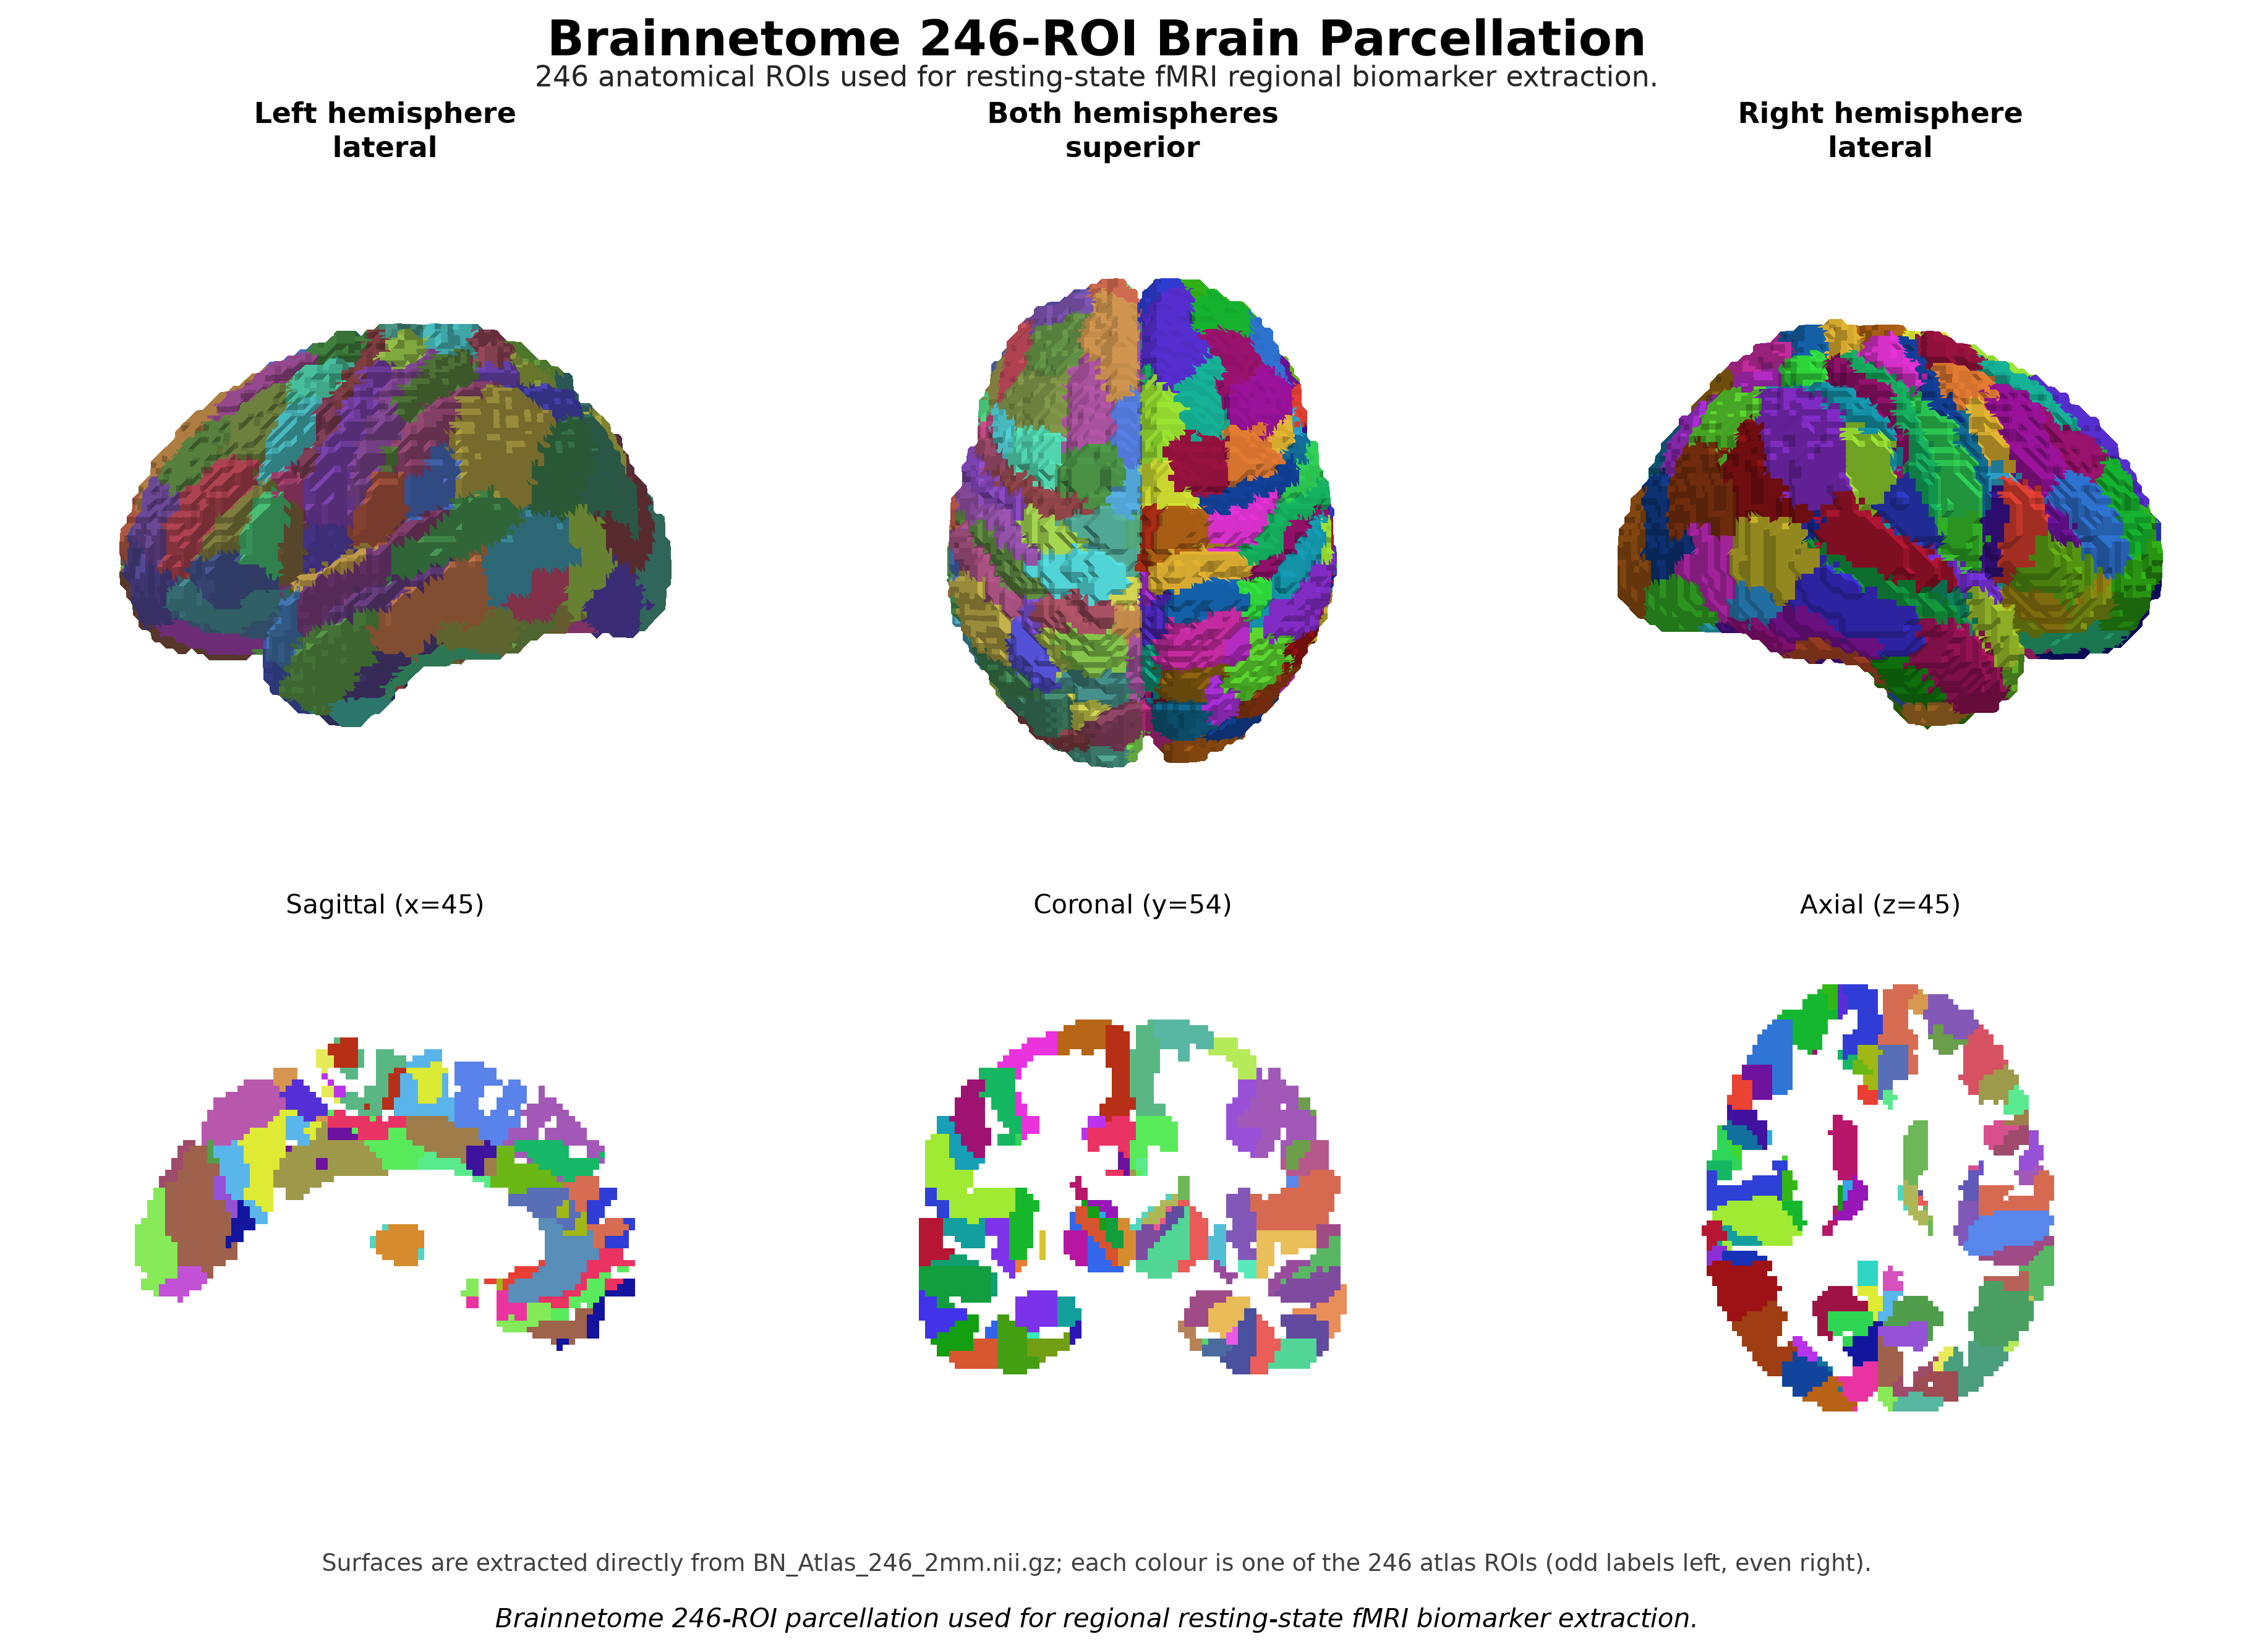
\includegraphics[width=\textwidth]{brainnetome246_combined.png}
\end{column}
\begin{column}{0.52\textwidth}
\small
\begin{itemize}
  \item \textbf{Fine-grained whole-brain coverage.} 246 anatomically
        defined regions (210 cortical, 36 subcortical) with boundaries
        derived from structural connectivity, not sulcal landmarks alone.
  \item \textbf{A verified, complete extraction space.} 246/246 regions
        present in all 165 acquisitions; 0 empty, 0 below 10 voxels,
        0 zero-variance time series, 0 NaN/Inf.
  \item \textbf{Systematic regional features.} The same four biomarkers
        (ALFF, ReHo, DC, FC) are computed for every region by the same
        procedure, giving a $135\times246$ signal matrix and a
        $246\times246$ connectivity matrix per scan.
  \item \textbf{No premature feature selection.} Regional and
        inter-regional information is preserved at extraction time;
        which regions and interactions are predictive is decided later,
        by the model.
\end{itemize}
\end{column}
\end{columns}

\vspace{0.1cm}
\begin{block}{Position}
We do not claim every region is individually disease-relevant. We retain the
complete 246-region representation so that nothing is discarded before the
predictive model can evaluate it.
\end{block}

\end{frame}


% ---------------------------------------------------------------- BACKUP
\begin{frame}{Backup: The 246-ROI Extraction Space Is Verified}
\begin{center}
  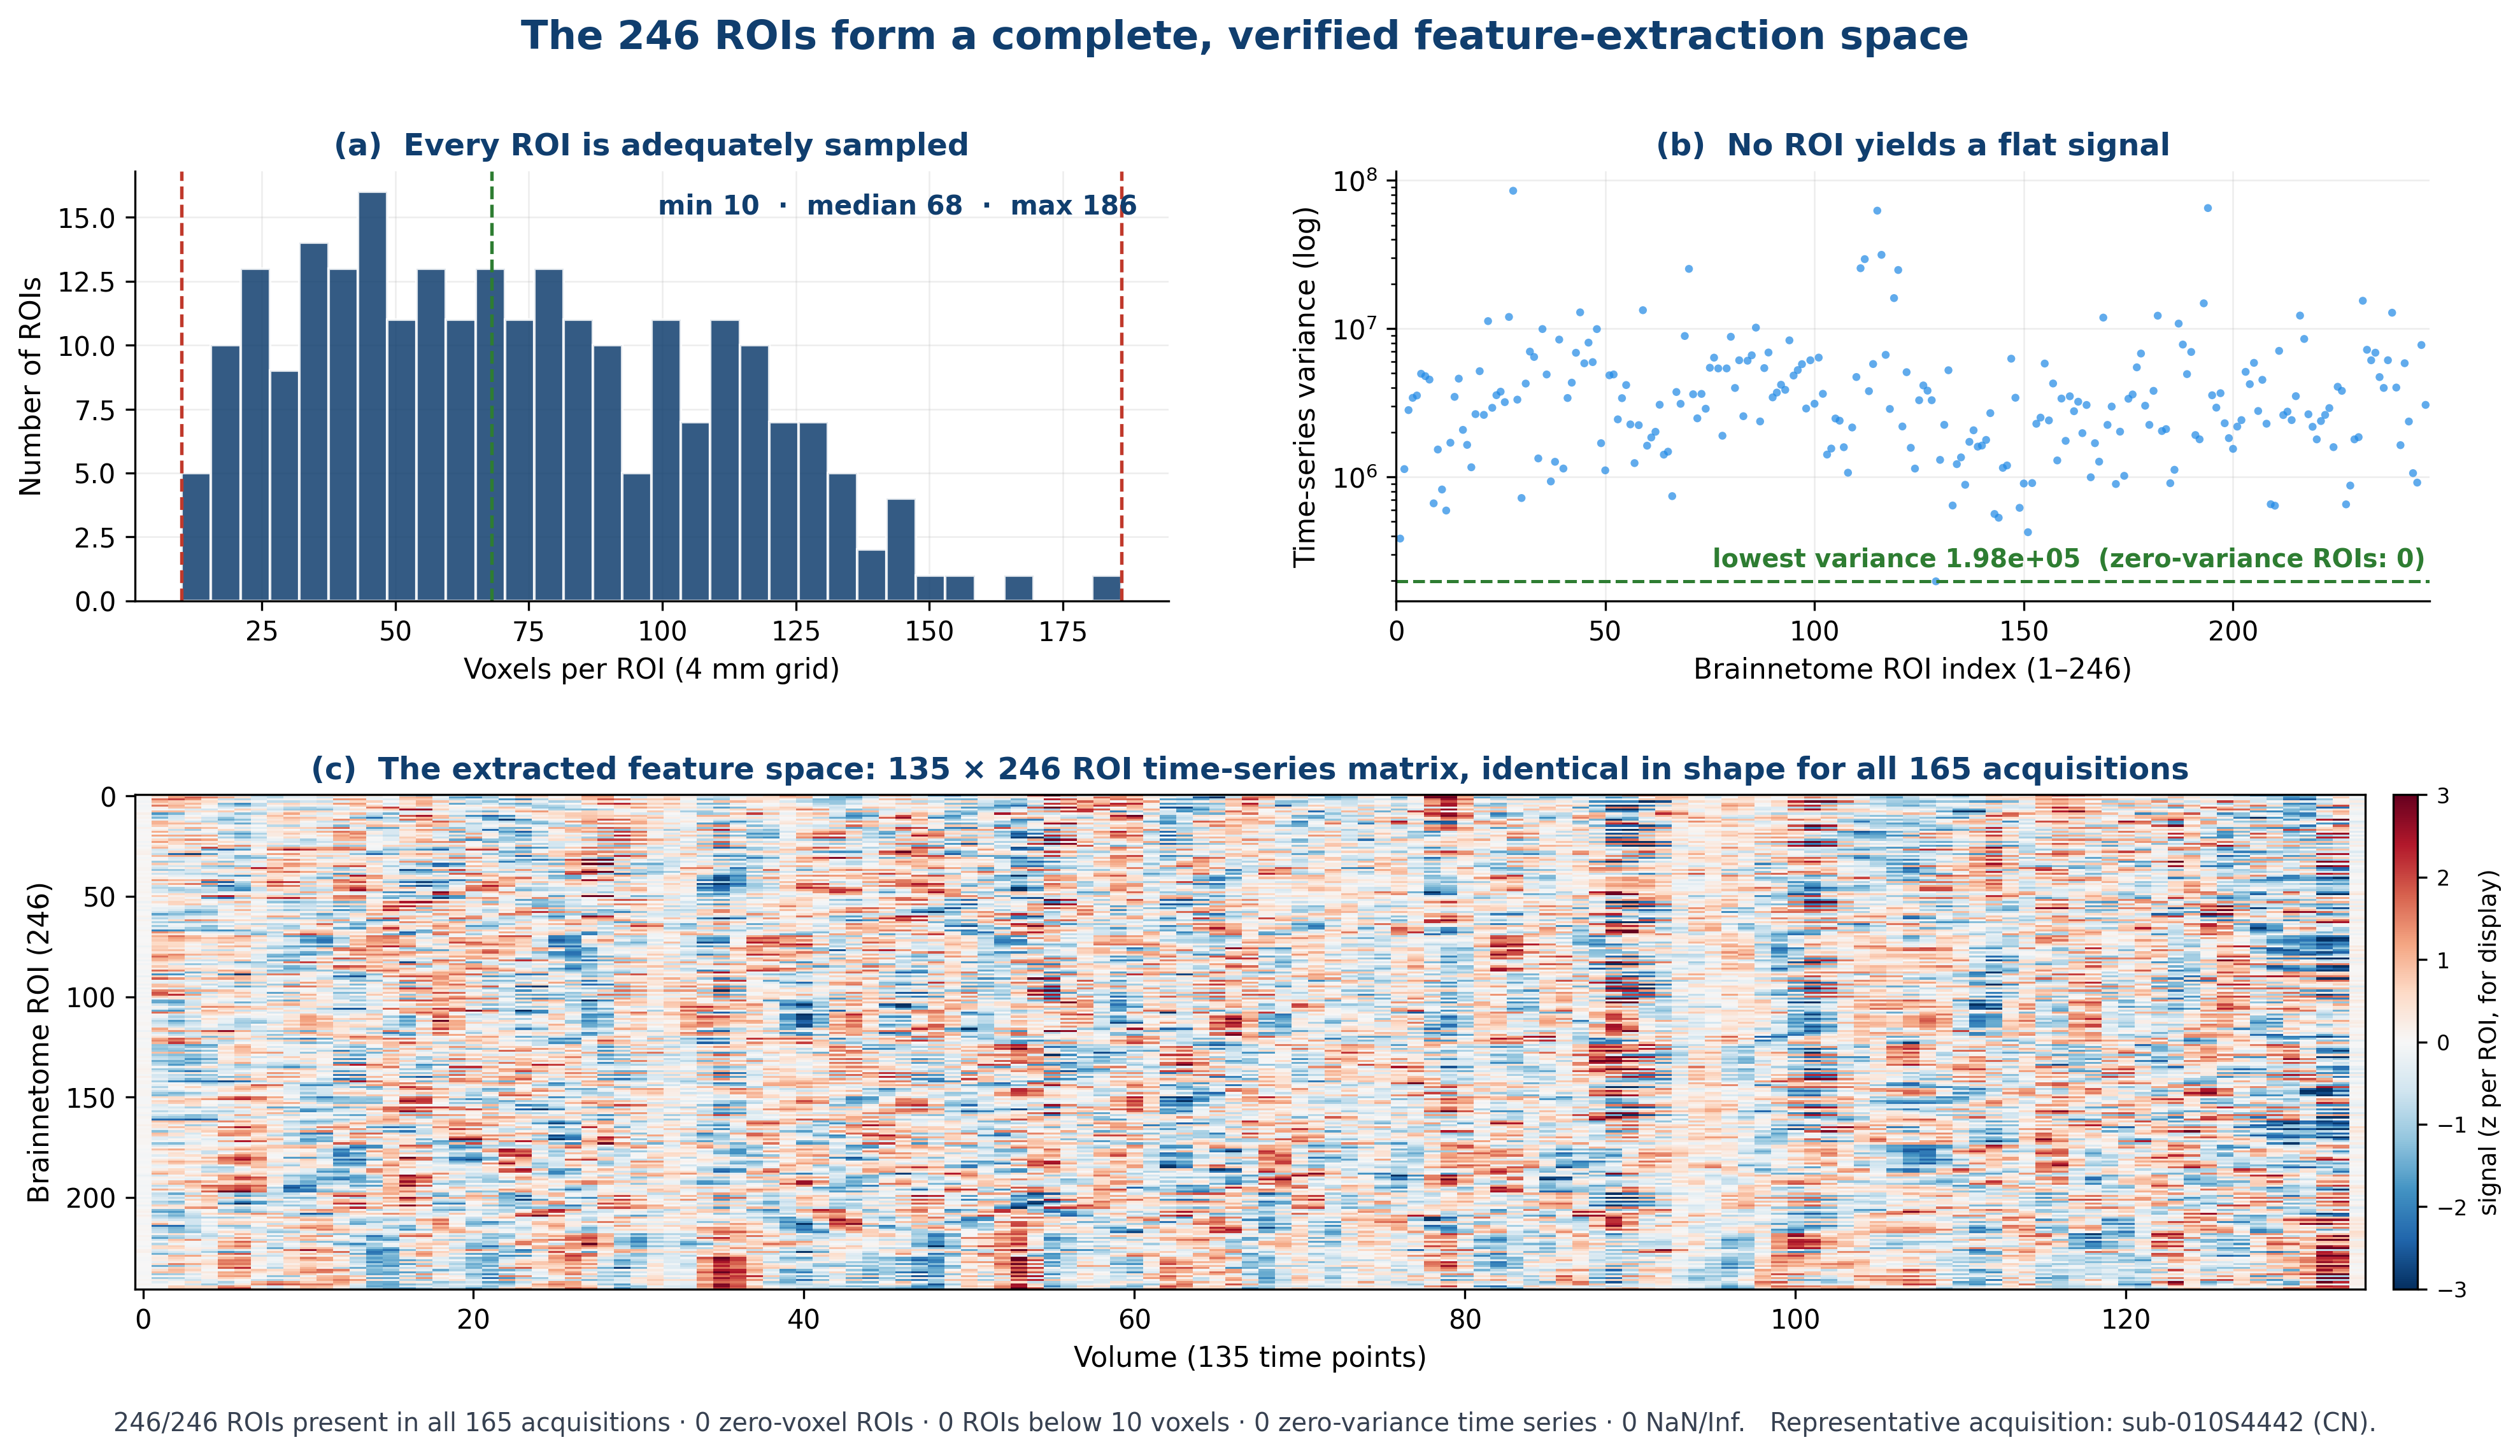
\includegraphics[width=0.93\textwidth]{fig_roi_qc.png}
\end{center}
\end{frame}


\begin{frame}{Backup: 246 Regions as Connectivity Nodes}
\begin{center}
  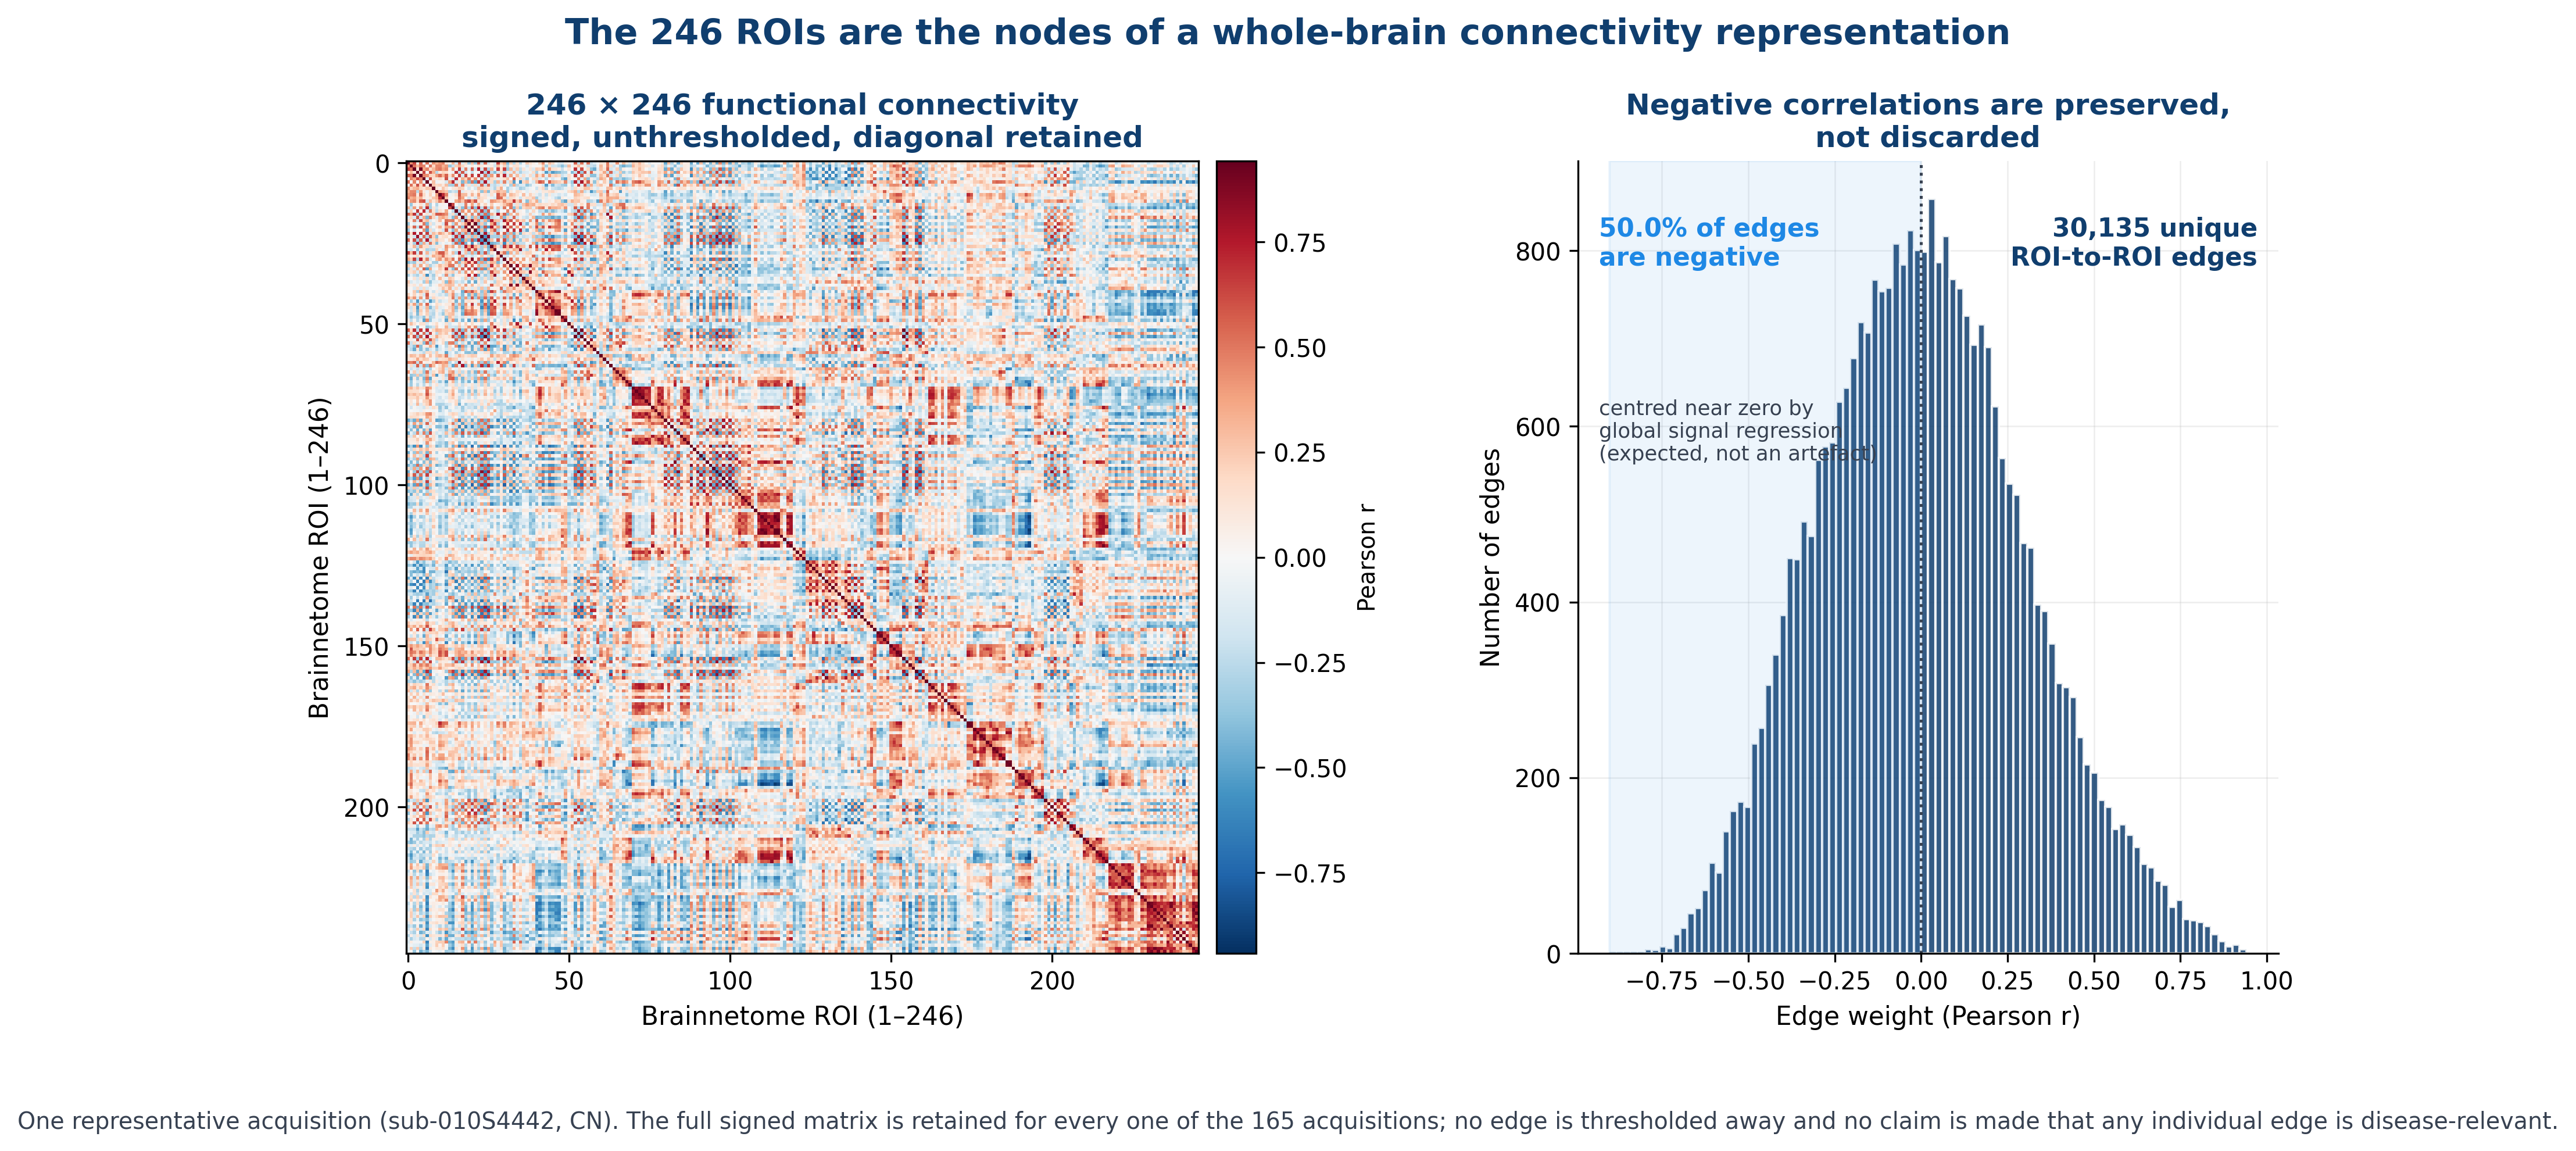
\includegraphics[width=0.95\textwidth]{fig_fc_matrix.png}
\end{center}
\vspace{-0.2cm}
{\footnotesize Signed and unthresholded: 30{,}135 unique edges, of which
50.1\,\% are negative across the cohort. The distribution is centred near zero
because global signal regression is part of the 27-regressor design --
expected, and documented as a known trade-off.}
\end{frame}
